\chapter{Технологическая часть}

\section{Выбор операционной системы}

Согласно требованиям технического задания, разрабатываемая система должна запускаться в среде оркестрации Kubernetes. Для узлов кластера была выбрана операционная система Linux, дистрибутив Ubuntu. \textbf{Ubuntu} \cite{ubuntu} является распространенным серверным дистрибутивом, поддерживает контейнеризацию, имеет развитую экосистему пакетов и широко применяется при развертывании микросервисных систем.

\section{Выбор СУБД}

В качестве СУБД была выбрана \textbf{PostgreSQL} \cite{postgresql}. Данная СУБД используется сервисами автомобилей, бронирований, платежей, авторизации и статистики. Каждый сервис работает со своей логической базой данных:

\begin{itemize}
  \item база \texttt{cars} хранит автомобили;
  \item база \texttt{rentals} хранит бронирования;
  \item база \texttt{payments} хранит платежи;
  \item база \texttt{identity} хранит учетные записи пользователей;
  \item база \texttt{statistics} хранит события системы.
\end{itemize}

PostgreSQL была выбрана из-за поддержки транзакций, надежности, удобной работы с UUID и распространенности в микросервисных приложениях.

\section{Выбор языка разработки и backend-фреймворка}

Для разработки backend-сервисов был выбран \textbf{Python} \cite{python}. Данный язык позволяет быстро создавать прототипы, имеет развитую экосистему библиотек для работы с HTTP API, базами данных, JWT и Kafka.

В качестве backend-фреймворка был выбран \textbf{FastAPI} \cite{fastapi}. Он подходит для реализации микросервисов по следующим причинам:

\begin{itemize}
  \item высокая скорость разработки REST API;
  \item поддержка декларативной валидации входных данных;
  \item автоматическая генерация OpenAPI-описания;
  \item удобная интеграция с middleware авторизации;
  \item поддержка асинхронной обработки запросов.
\end{itemize}

\section{Выбор фреймворка пользовательского интерфейса}

Для реализации пользовательского интерфейса был выбран \textbf{React} \cite{react}. Интерфейс реализован как Single Page Application, отдаваемое ui-service. React позволяет строить интерактивные страницы без перезагрузки, динамически обновлять список автомобилей, бронирований и административные отчеты.

\section{Асинхронное взаимодействие}

Для асинхронного взаимодействия между сервисами используется \textbf{Apache Kafka} \cite{kafka}. Gateway-service отправляет события о действиях пользователя в Kafka topic \texttt{car-rental-events}. Statistics-service читает эти события, сохраняет их в своей базе данных и строит отчет для администратора.

Через Kafka передаются следующие типы событий:

\begin{itemize}
  \item регистрация пользователя;
  \item создание бронирования;
  \item завершение бронирования;
  \item отмена бронирования.
\end{itemize}

\section{Реализация микросервисов}

Система состоит из следующих сервисов.

\subsection{UI-service}

UI-service отдает HTML-страницу с React-приложением. Пользовательский интерфейс содержит:

\begin{itemize}
  \item экран входа и регистрации;
  \item список автомобилей;
  \item выбор дат аренды;
  \item расчет стоимости;
  \item список бронирований пользователя;
  \item административную панель со списком пользователей и статистикой.
\end{itemize}

\subsection{Identity-service}

Identity-service выполняет роль собственного Identity Provider \cite{idprovider}. Сервис реализует Authorization Code Flow, выдачу JWT, JWKs, регистрацию пользователей, создание пользователей администратором и ролевую модель Admin/User.

При старте сервиса автоматически создается администратор. Новые пользователи, созданные через регистрацию или администратором, получают роль User.

\subsection{Cars-service}

Cars-service отвечает за хранение и выдачу данных об автомобилях. Для каждого автомобиля хранится марка, модель, регистрационный номер, мощность, цена за день, тип и признак доступности. Сервис предоставляет методы получения списка автомобилей, получения автомобиля по идентификатору и изменения доступности автомобиля.

\subsection{Rental-service}

Rental-service отвечает за бронирования. Сервис хранит идентификатор бронирования, пользователя, автомобиль, платеж, даты начала и окончания аренды, а также статус. Возможные статусы: IN\_PROGRESS, FINISHED, CANCELED.

\subsection{Payment-service}

Payment-service отвечает за платежи. При создании бронирования gateway-service создает платеж на рассчитанную сумму. Платеж может находиться в статусе PAID или CANCELED.

\subsection{Statistics-service}

Statistics-service получает события из Kafka, сохраняет их в БД и предоставляет административные методы получения сводки и списка событий. Доступ к данным статистики разрешен только пользователю с ролью Admin.

\subsection{Gateway-service}

Gateway-service является сервисом агрегирования запросов. Он принимает запросы от UI и внешних клиентов, валидирует JWT, вызывает внутренние сервисы и формирует агрегированные ответы. Например, при получении списка бронирований gateway-service добавляет к бронированию сведения об автомобиле и платеже.

\section{Авторизация и межсервисное взаимодействие}

Все сервисы используют общий middleware для проверки JWT. Токен передается в заголовке \texttt{Authorization: Bearer}. Валидация выполняется по JWKs. При ошибке авторизации сервис возвращает HTTP 401.

Gateway-service пробрасывает JWT во внутренние сервисы. Таким образом, межсервисные запросы также защищены token-based авторизацией, а пользователь определяется из claims JWT.

\section{Обработка ошибок и деградация}

В системе предусмотрена обработка ошибок зависимых сервисов. Если сервис статистики или Kafka временно недоступны, основная пользовательская операция не блокируется. При недоступности платежного сервиса gateway-service использует механизм деградации для сохранения работоспособности сценариев бронирования и отмены. Ошибки сервисов преобразуются в корректные HTTP-ответы с соответствующими статусами.

\section{Логирование}

Во всех сервисах добавлено логирование входящих HTTP-запросов: метод, путь, статус ответа и время выполнения. Gateway-service также логирует ключевые бизнес-события и отправляет их в Kafka для последующей обработки statistics-service.

\section{Развертывание}

Все сервисы контейнеризуются и разворачиваются в Kubernetes \cite{kubernetes}. Для развертывания используется универсальный Helm chart \texttt{service-chart} \cite{helm}. Отличия между сервисами задаются через values-файлы:

\begin{itemize}
  \item \texttt{identity-service.yaml};
  \item \texttt{ui-service.yaml};
  \item \texttt{cars-service.yaml};
  \item \texttt{rental-service.yaml};
  \item \texttt{payment-service.yaml};
  \item \texttt{statistics-service.yaml};
  \item \texttt{gateway-service.yaml};
  \item \texttt{kafka.yaml}.
\end{itemize}

PostgreSQL разворачивается отдельным Helm chart \texttt{postgres-chart}, который создает базу данных и job инициализации схем.

Для публикации сервисов наружу используется Ingress Controller \texttt{ingress-nginx}. Наружу публикуются только:

\begin{itemize}
  \item \texttt{/} --- пользовательский интерфейс;
  \item \texttt{/api} и \texttt{/manage} --- gateway-service;
  \item \texttt{/oauth} и \texttt{/.well-known} --- identity-service.
\end{itemize}

\section{CI/CD}

Сборка и развертывание выполняются через GitHub Actions. Pipeline выполняет следующие шаги:

\begin{enumerate}
  \item запуск unit-тестов;
  \item сборка Docker-образов сервисов;
  \item публикация Docker-образов;
  \item развертывание PostgreSQL, Kafka и сервисов в Kubernetes через Helm;
  \item запуск Newman-тестов для проверки Gateway API.
\end{enumerate}

\section{Высокоуровневый дизайн пользовательского интерфейса}

Пользовательский интерфейс системы представляет собой веб-интерфейс, доступный через браузер. Основные страницы системы:

\begin{itemize}
  \item страница входа и регистрации;
  \item страница списка автомобилей;
  \item страница бронирований пользователя;
  \item страница администрирования;
  \item страница статистики.
\end{itemize}

Примеры страниц приведены на рисунках \ref{fig:page-01}-\ref{fig:page-08}.

\begin{figure}[H]
	\begin{center}
		{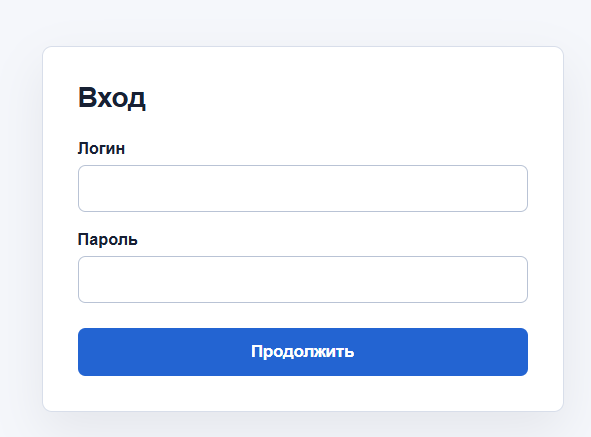
\includegraphics[width=\textwidth,height=0.78\textheight,keepaspectratio]{../img/pages/page-01.png}}
		\caption{Страница входа}
		\label{fig:page-01}
	\end{center}
\end{figure}

\begin{figure}[H]
	\begin{center}
		{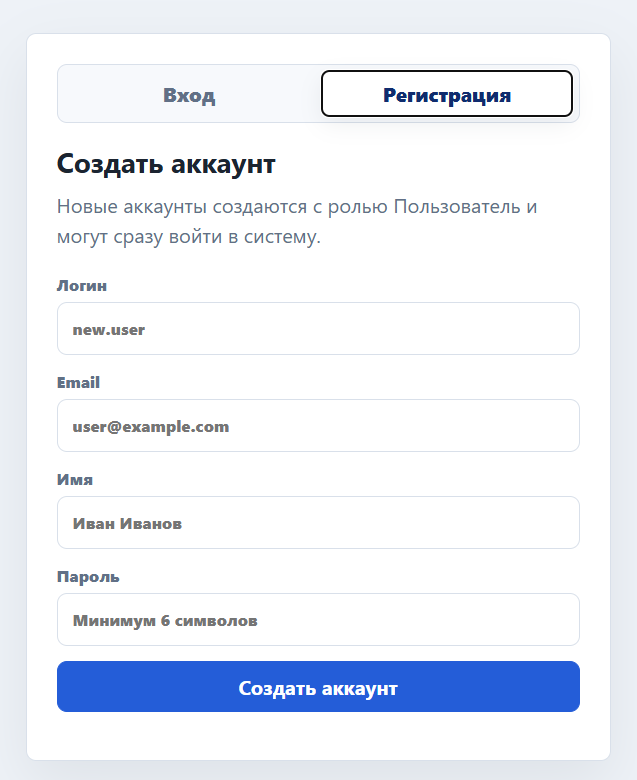
\includegraphics[width=\textwidth,height=0.78\textheight,keepaspectratio]{../img/pages/page-02.png}}
		\caption{Страница регистрации}
		\label{fig:page-02}
	\end{center}
\end{figure}

\begin{figure}[H]
	\begin{center}
		{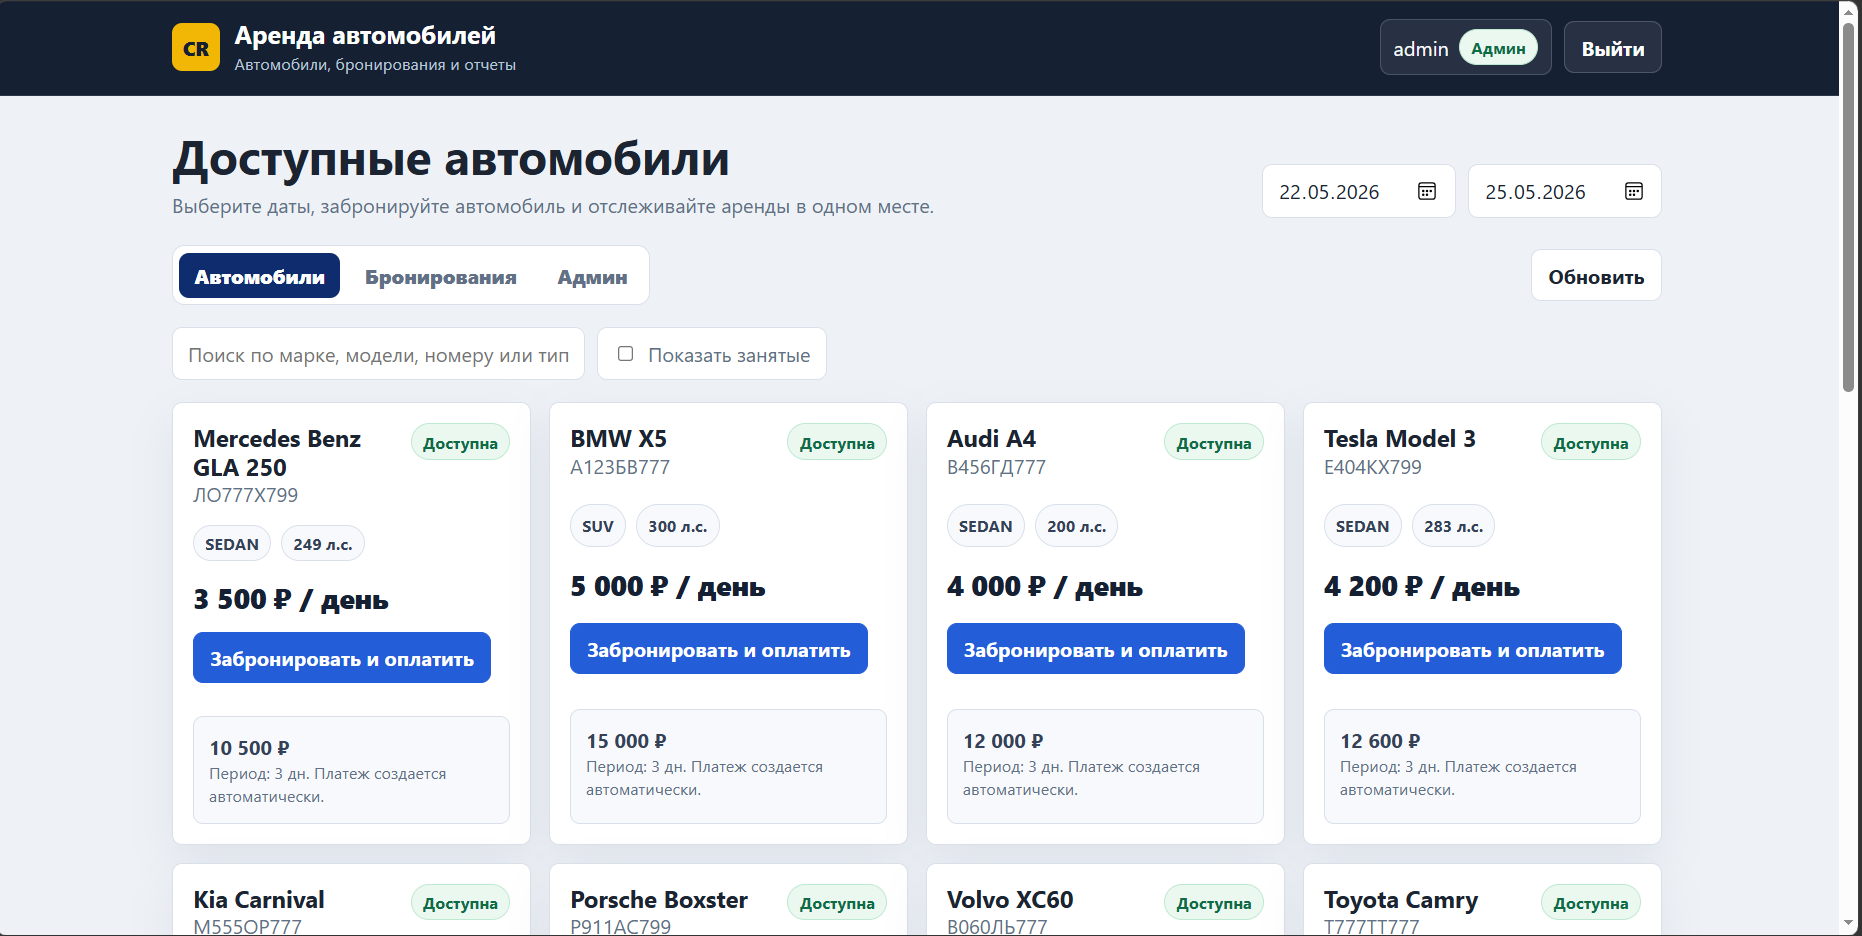
\includegraphics[width=\textwidth,height=0.78\textheight,keepaspectratio]{../img/pages/page-03.png}}
		\caption{Страница списка автомобилей}
		\label{fig:page-03}
	\end{center}
\end{figure}

\begin{figure}[H]
	\begin{center}
		{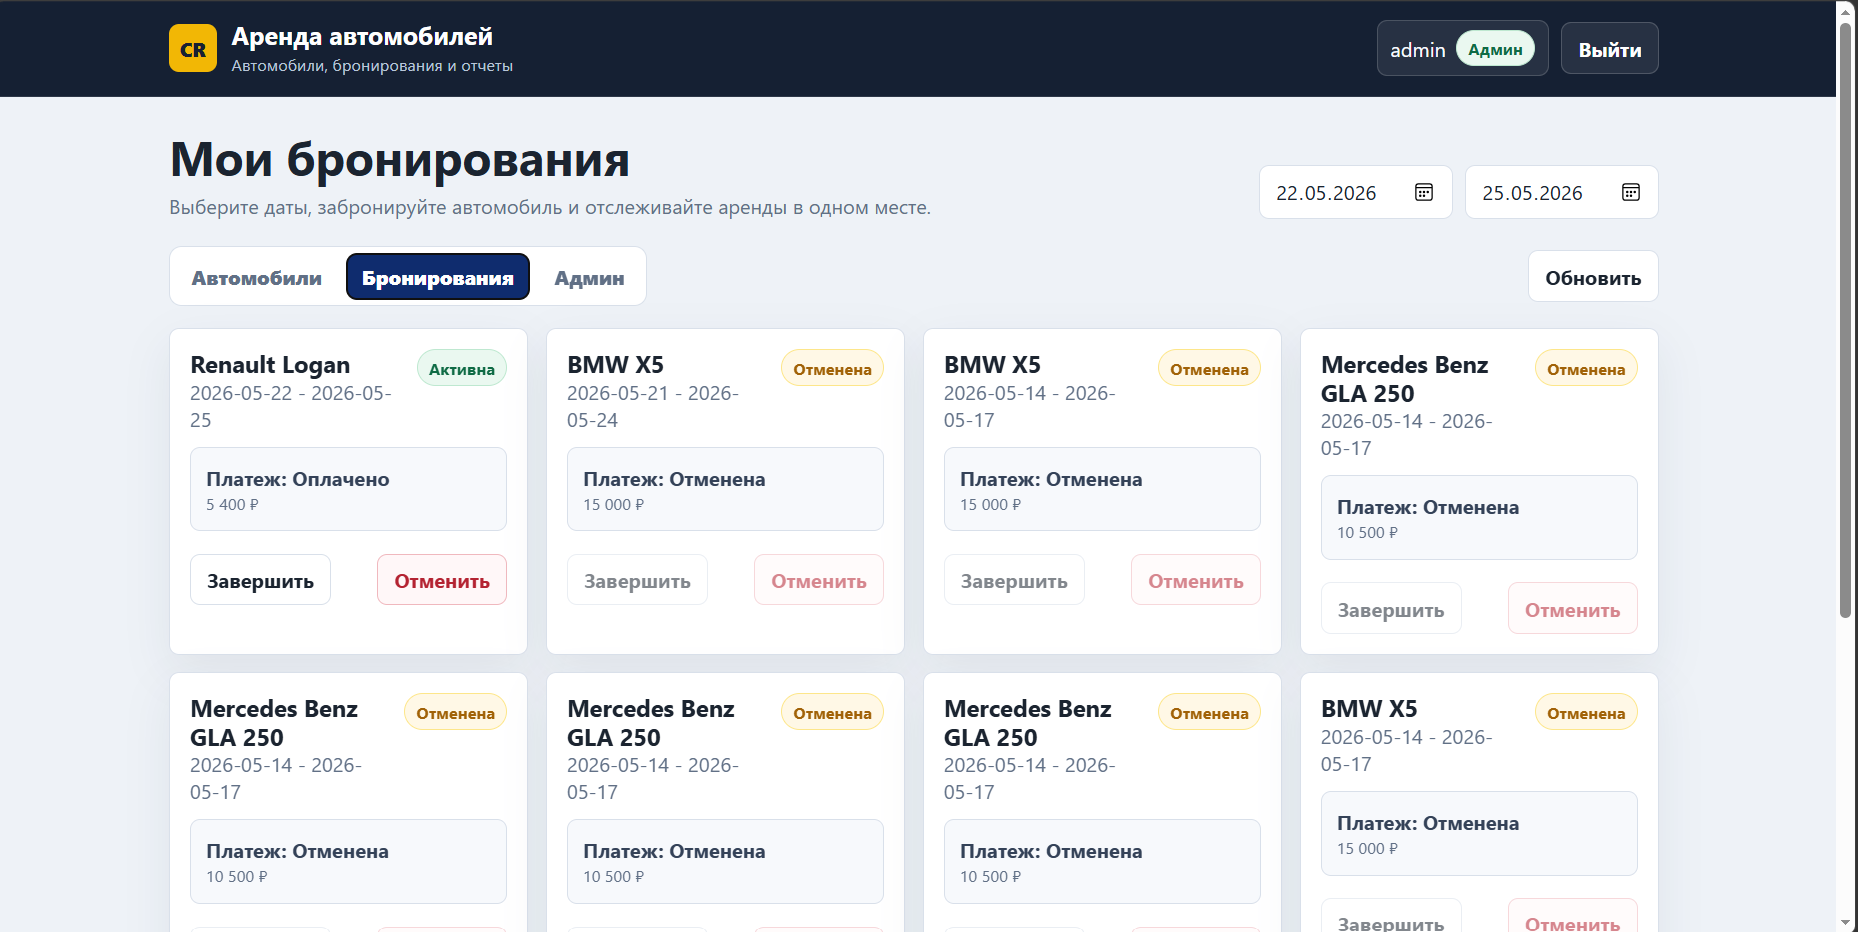
\includegraphics[width=\textwidth,height=0.78\textheight,keepaspectratio]{../img/pages/page-04.png}}
		\caption{Страница бронирования автомобиля}
		\label{fig:page-04}
	\end{center}
\end{figure}

\begin{figure}[H]
	\begin{center}
		{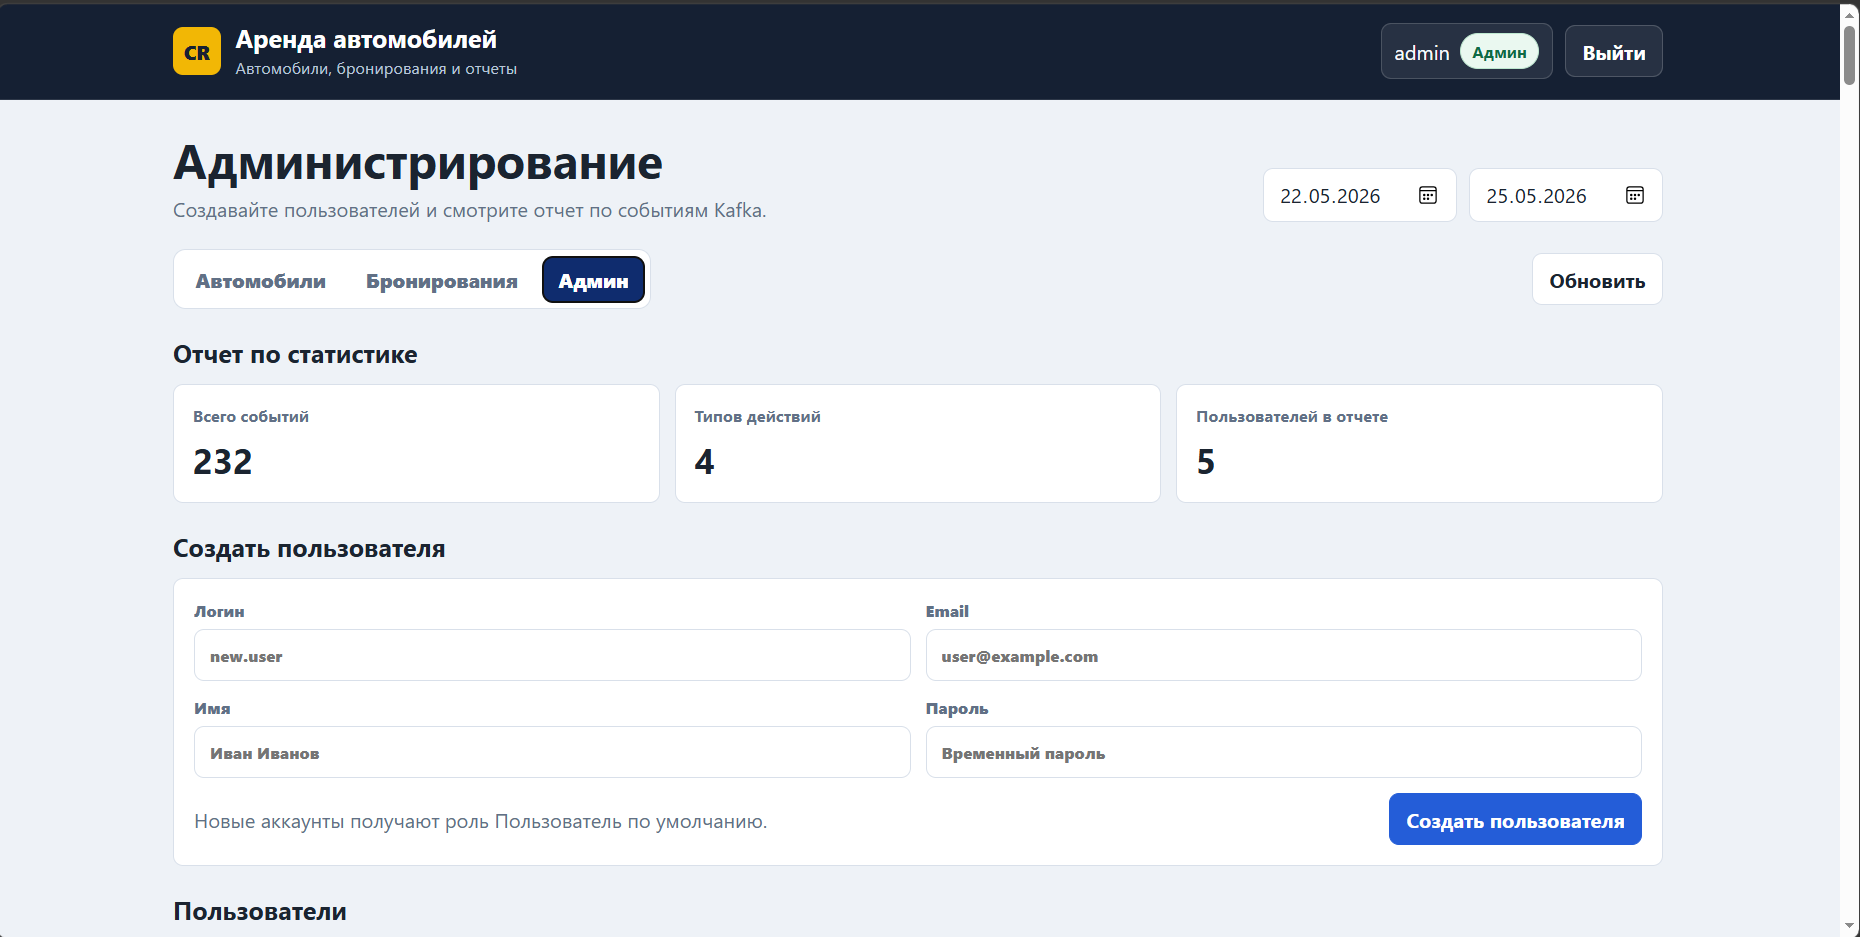
\includegraphics[width=\textwidth,height=0.78\textheight,keepaspectratio]{../img/pages/page-05.png}}
		\caption{Страница бронирований пользователя}
		\label{fig:page-05}
	\end{center}
\end{figure}

\begin{figure}[H]
	\begin{center}
		{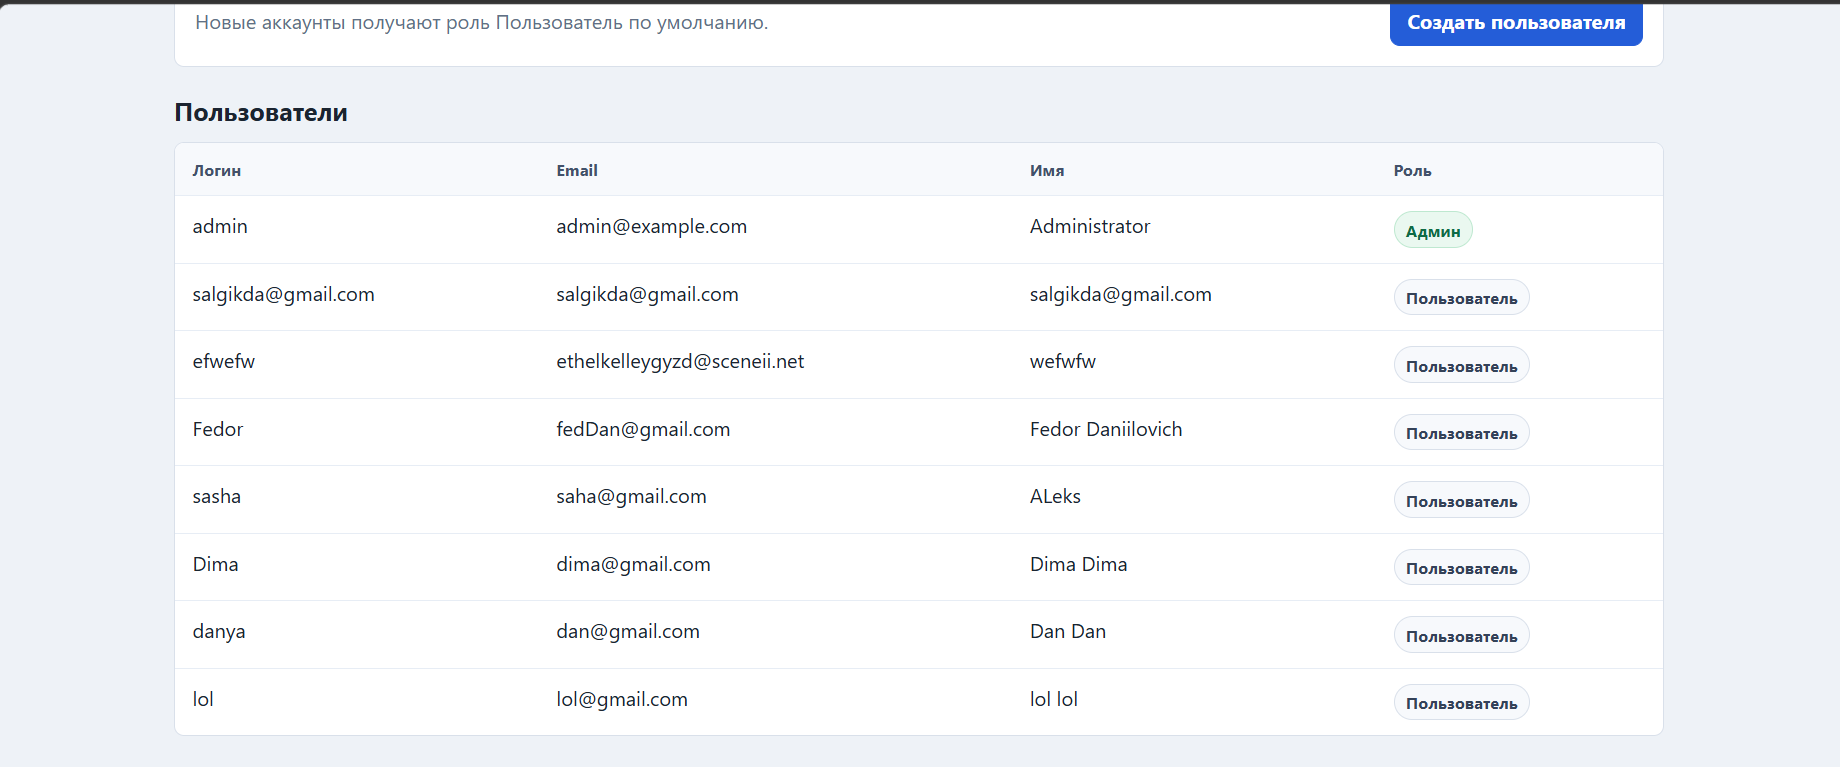
\includegraphics[width=\textwidth,height=0.78\textheight,keepaspectratio]{../img/pages/page-06.png}}
		\caption{Страница администрирования пользователей}
		\label{fig:page-06}
	\end{center}
\end{figure}

\begin{figure}[H]
	\begin{center}
		{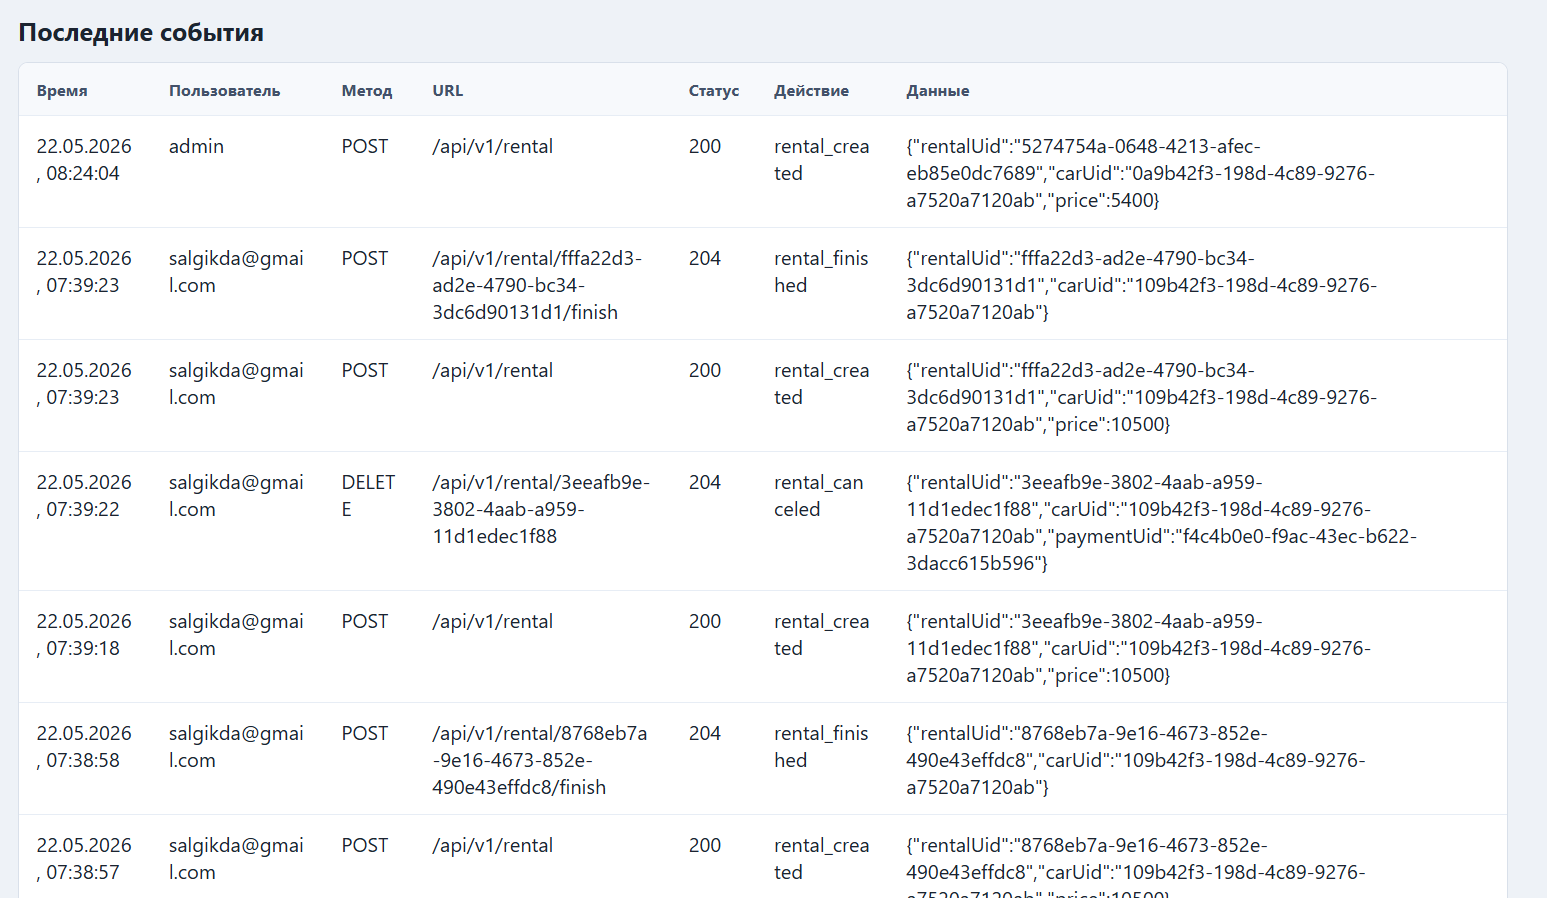
\includegraphics[width=\textwidth,height=0.78\textheight,keepaspectratio]{../img/pages/page-07.png}}
		\caption{Страница статистики}
		\label{fig:page-07}
	\end{center}
\end{figure}

\begin{figure}[H]
	\begin{center}
		{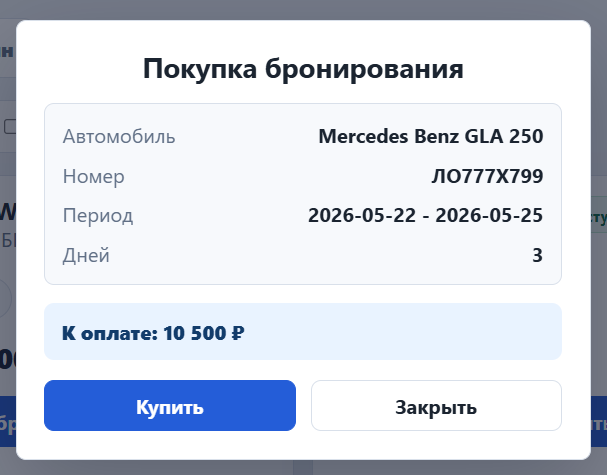
\includegraphics[width=\textwidth,height=0.78\textheight,keepaspectratio]{../img/pages/page-08.png}}
		\caption{Окно подтверждения покупки бронирования}
		\label{fig:page-08}
	\end{center}
\end{figure}

\section{Вывод}

В технологической части были выбраны основные технологии реализации, описаны микросервисы системы, механизм авторизации, обработка ошибок, логирование, развертывание в Kubernetes и CI/CD pipeline.
